% !TEX program = pdflatex
\documentclass[aspectratio=169,11pt]{beamer}

\usetheme{Madrid}
\usecolortheme{seahorse}
\setbeamertemplate{navigation symbols}{}
\setbeamertemplate{footline}[frame number]

\usepackage[T1]{fontenc}
\usepackage{lmodern}
\usepackage{listings}
\usepackage{booktabs}
\usepackage{tikz}
\usetikzlibrary{arrows.meta,positioning}

\lstset{
  basicstyle=\ttfamily\scriptsize,
  keywordstyle=\color{blue!70!black}\bfseries,
  commentstyle=\color{green!50!black},
  stringstyle=\color{red!60!black},
  breaklines=true,
  showstringspaces=false,
  columns=fullflexible,
  frame=single,
  backgroundcolor=\color{gray!8},
  rulecolor=\color{gray!40},
  xleftmargin=2pt,
  xrightmargin=2pt,
}

\definecolor{beastblue}{RGB}{40,80,140}
\definecolor{beastorange}{RGB}{200,100,20}
\setbeamercolor{frametitle}{fg=beastblue}
\setbeamercolor{title}{fg=beastblue}
\setbeamercolor{structure}{fg=beastblue}

\newcommand{\pkg}[1]{\texttt{\color{beastorange}#1}}
\newcommand{\code}[1]{\texttt{#1}}
\newcommand{\deprecated}[1]{\textcolor{red!60!black}{\sout{#1}}}

\usepackage[normalem]{ulem} % for \sout

\title{BEAST 3: What's New for Package Developers}
\author{BEAST Core Developer Team}
\date{2026}

\begin{document}

% ============================================================
% TITLE & OVERVIEW
% ============================================================

\begin{frame}
\titlepage
\end{frame}

\begin{frame}{Outline}
\tableofcontents
\end{frame}

\begin{frame}{The Big Picture}
Three pillars of change in BEAST 3:
\vspace{1em}
\begin{enumerate}
\item \textbf{Maven + JPMS} --- modern build system and module isolation
\item \textbf{Strongly-typed spec system} --- compile-time checked inputs and domain types
\item \textbf{New package distribution} --- Maven Central JARs, module-based service discovery
\end{enumerate}
\vspace{1em}
\begin{block}{Goal}
Catch more errors at compile time, simplify dependency management, and make packages first-class citizens in the Java module system.
\end{block}
\end{frame}

% ============================================================
\section{Build \& Tooling}
% ============================================================

\begin{frame}{Ant $\to$ Maven}
\begin{columns}[T]
\begin{column}{0.48\textwidth}
\textbf{BEAST 2}
\begin{itemize}
\item Ant \code{build.xml}
\item Manual JAR management
\item One monolithic project
\item Classpath-based
\end{itemize}
\end{column}
\begin{column}{0.48\textwidth}
\textbf{BEAST 3}
\begin{itemize}
\item Maven \code{pom.xml}
\item Automatic dependency resolution
\item Multi-module project
\item Module-path-based (JPMS)
\end{itemize}
\end{column}
\end{columns}
\end{frame}

\begin{frame}{Java 25 + JPMS Modules}
\begin{itemize}
\item Requires \textbf{JDK 25} (was Java 8/11)
\item JavaFX is a \textbf{Maven dependency} --- no bundled JDK needed
\item Three JPMS modules, each with \code{module-info.java}:
\end{itemize}
\vspace{0.5em}
\begin{center}
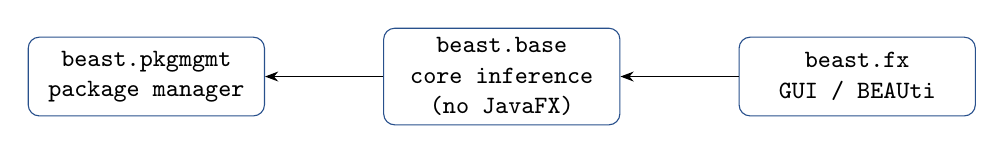
\begin{tikzpicture}[
    box/.style={draw=beastblue, rounded corners, minimum width=3cm, minimum height=1cm, align=center, font=\small\ttfamily},
    >=Stealth
]
\node[box] (pkgmgmt) {\textbf{beast.pkgmgmt}\\package manager};
\node[box, right=1.5cm of pkgmgmt] (base) {\textbf{beast.base}\\core inference\\(no JavaFX)};
\node[box, right=1.5cm of base] (fx) {\textbf{beast.fx}\\GUI / BEAUti};
\draw[->] (base) -- (pkgmgmt);
\draw[->] (fx) -- (base);
\end{tikzpicture}
\end{center}
\vspace{0.5em}
All declared as \code{open module} (reflection OK for XML unmarshalling).
\end{frame}

\begin{frame}{Project Structure}
\begin{center}
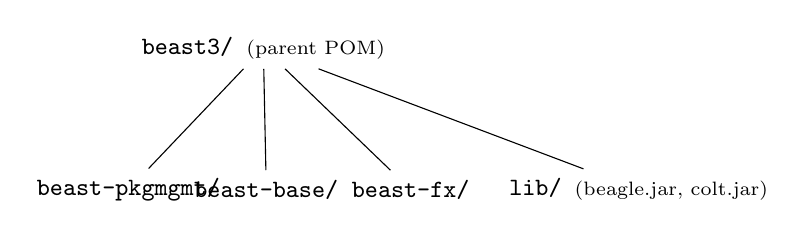
\begin{tikzpicture}[
    every node/.style={font=\small\ttfamily, anchor=west},
    level 1/.style={sibling distance=2cm, level distance=1.8cm},
]
\node {\textbf{beast3/} \textrm{\scriptsize(parent POM)}}
  child {node {beast-pkgmgmt/}}
  child {node {beast-base/}}
  child {node {beast-fx/}}
  child {node {lib/ \textrm{\scriptsize(beagle.jar, colt.jar)}}};
\end{tikzpicture}
\end{center}
\vspace{1em}
\begin{itemize}
\item \code{beast-base} has \textbf{no JavaFX dependency} --- can be used headlessly
\item \code{beagle} and \code{colt} ship as modular JARs in \code{lib/}
\end{itemize}
\end{frame}

\begin{frame}{What This Means for Your Package}
\begin{enumerate}
\item \textbf{Recommended:} create a Maven \code{pom.xml} for your package
  \begin{itemize}
  \item See \pkg{beast-package-skeleton} on GitHub
  \end{itemize}
\item \textbf{Alternative:} keep Ant, but update classpath JARs
\item Add a \code{module-info.java} with \code{provides} declarations
\item Target \textbf{Java 25} (use \code{--release 25})
\end{enumerate}
\vspace{1em}
\begin{alertblock}{Tip}
The \pkg{beast-package-skeleton} repo is a ready-to-copy Maven project with all of this pre-configured.
\end{alertblock}
\end{frame}

% ============================================================
\section{Strongly Typed Spec System}
% ============================================================

\begin{frame}{Why Types?}
\textbf{Problem:} In BEAST 2, almost everything is \code{Input<RealParameter>} or \code{Input<Function>}
\begin{itemize}
\item Type errors discovered at \textbf{runtime} (wrong parameter passed to wrong input)
\item Bounds (\code{lower="0"}) are stringly-typed XML attributes
\item No way to express ``this must be a positive real'' in the Java API
\end{itemize}
\vspace{1em}
\textbf{Solution:} New \code{beast.base.spec} hierarchy
\begin{itemize}
\item Compile-time checked typed inputs
\item Domain types encode valid ranges
\item Self-documenting model structure
\end{itemize}
\end{frame}

\begin{frame}{Parameter Types}
\code{RealParameter} is replaced by specific types:
\vspace{0.5em}

\begin{center}
\begin{tabular}{lll}
\toprule
\textbf{BEAST 2} & \textbf{BEAST 3} & \textbf{Use for} \\
\midrule
\code{RealParameter} (dim=1) & \code{RealScalarParam} & single real value \\
\code{RealParameter} (dim$>$1) & \code{RealVectorParam} & vector of reals \\
\code{IntegerParameter} & \code{IntScalarParam} / \code{IntVectorParam} & integer values \\
\code{BooleanParameter} & \code{BoolScalarParam} / \code{BoolVectorParam} & boolean values \\
\code{RealParameter} (simplex) & \code{SimplexParam} & probability simplex \\
\bottomrule
\end{tabular}
\end{center}
\end{frame}

\begin{frame}{Domain Types}
Domains replace explicit \code{lower}/\code{upper} bounds:
\vspace{0.5em}

\begin{center}
\begin{tabular}{ll}
\toprule
\textbf{BEAST 2 XML pattern} & \textbf{BEAST 3 domain} \\
\midrule
\code{RealParameter lower="0"} & \code{PositiveReal.INSTANCE} \\
\code{RealParameter lower="0" upper="1"} & \code{UnitInterval.INSTANCE} \\
\code{RealParameter} (unbounded) & \code{Real.INSTANCE} \\
\code{IntegerParameter lower="0"} & \code{NonNegativeInt.INSTANCE} \\
\code{IntegerParameter lower="1"} & \code{PositiveInt.INSTANCE} \\
\bottomrule
\end{tabular}
\end{center}
\vspace{0.5em}
Domains propagate through the model graph at initialization time.
\end{frame}

\begin{frame}{``Distribution IS the Prior''}
\begin{columns}[T]
\begin{column}{0.48\textwidth}
\textbf{BEAST 2}

\medskip
\code{Prior} wraps distribution + parameter:

\begin{center}
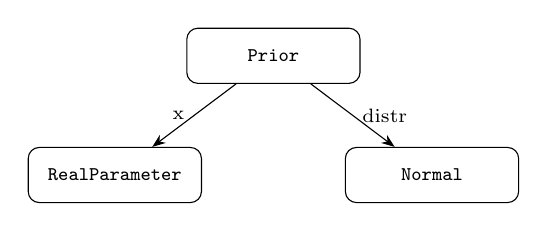
\begin{tikzpicture}[
    box/.style={draw, rounded corners, minimum width=2.2cm, minimum height=0.7cm, font=\scriptsize\ttfamily, align=center},
    >=Stealth, scale=0.9
]
\node[box] (prior) {Prior};
\node[box, below left=0.8cm and -0.2cm of prior] (param) {RealParameter};
\node[box, below right=0.8cm and -0.2cm of prior] (dist) {Normal};
\draw[->] (prior) -- node[left, font=\scriptsize]{x} (param);
\draw[->] (prior) -- node[right, font=\scriptsize]{distr} (dist);
\end{tikzpicture}
\end{center}
\end{column}
\begin{column}{0.48\textwidth}
\textbf{BEAST 3}

\medskip
Distribution \textbf{is} the prior:

\begin{center}
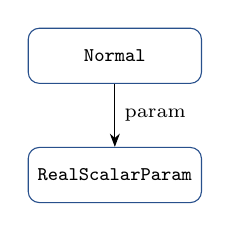
\begin{tikzpicture}[
    box/.style={draw=beastblue, rounded corners, minimum width=2.2cm, minimum height=0.7cm, font=\scriptsize\ttfamily, align=center},
    >=Stealth, scale=0.9
]
\node[box] (normal) {Normal};
\node[box, below=0.8cm of normal] (param) {RealScalarParam};
\draw[->] (normal) -- node[right, font=\scriptsize]{param} (param);
\end{tikzpicture}
\end{center}
\end{column}
\end{columns}
\vspace{1em}
No separate \code{Prior} wrapper needed --- each distribution has a \code{param} input directly (from \code{TensorDistribution}).
\end{frame}

\begin{frame}[fragile]{Spec Classes Coexist with Legacy}
\begin{itemize}
\item Legacy classes are \textbf{deprecated}, not removed
\item Each deprecated class links to its spec replacement:
\end{itemize}

\begin{lstlisting}[language=Java]
/**
 * @deprecated use {@link RealScalarParam} or {@link RealVectorParam}
 */
public class RealParameter extends ...
\end{lstlisting}

\begin{itemize}
\item Your IDE shows deprecated usage (strikethrough)
\item \textbf{Migrate incrementally} --- old and new classes can coexist
\item Consider a \code{yourpackage.spec} sub-package for backward compatibility
\end{itemize}
\end{frame}

\begin{frame}[fragile]{Before / After: Input Declaration}
\begin{columns}[T]
\begin{column}{0.48\textwidth}
\textbf{BEAST 2}
\begin{lstlisting}[language=Java]
public Input<RealParameter> kappaInput =
    new Input<>("kappa",
    "ts/tv ratio",
    Validate.REQUIRED);
\end{lstlisting}
\end{column}
\begin{column}{0.48\textwidth}
\textbf{BEAST 3}
\begin{lstlisting}[language=Java]
public Input<RealScalar<PositiveReal>>
    kappaInput = new Input<>("kappa",
    "ts/tv ratio",
    Validate.REQUIRED);
\end{lstlisting}
\end{column}
\end{columns}

\vspace{1em}
\begin{itemize}
\item Domain (\code{PositiveReal}) is part of the type --- no runtime \code{lower="0"} needed
\item Compiler catches if someone passes a \code{UnitInterval} parameter where \code{PositiveReal} is expected
\end{itemize}
\end{frame}

\begin{frame}{When NOT to Use Spec Types}
\textbf{Spec parameters are for MCMC-estimated quantities only.}

\vspace{1em}
Keep plain \code{Input<Integer>}, \code{Input<Double>}, etc.\ for:
\begin{itemize}
\item Dimension counts
\item Category numbers
\item Boolean flags
\item Configuration / initializer values
\end{itemize}

\vspace{1em}
\begin{exampleblock}{Rule of thumb}
If it appears in the MCMC state, use a spec parameter type.\\
If it's fixed configuration, use a plain \code{Input<>}.
\end{exampleblock}
\end{frame}

% ============================================================
\section{New Distributions \& Operators}
% ============================================================

\begin{frame}{New Distributions}
Genuinely new --- not present in BEAST 2:

\vspace{0.5em}
\begin{columns}[T]
\begin{column}{0.48\textwidth}
\textbf{Continuous}
\begin{itemize}
\item \code{Cauchy} --- location / scale
\item \code{Laplace} --- $\mu$ / scale
\item \code{InverseGamma} --- $\alpha$ / $\beta$
\item \code{ChiSquare} --- degrees of freedom
\item \code{GammaMean} --- mean parameterization
\end{itemize}
\end{column}
\begin{column}{0.48\textwidth}
\textbf{Discrete \& Wrappers}
\begin{itemize}
\item \code{Bernoulli} --- boolean with prob $p$
\item \code{IntUniform} --- discrete uniform
\item \code{IID} --- scalar dist $\to$ vector
\item \code{OffsetReal} --- additive offset
\item \code{TruncatedReal} --- truncation bounds
\end{itemize}
\end{column}
\end{columns}
\end{frame}

\begin{frame}{New / Refactored Operators}
\begin{itemize}
\item \textbf{\code{IntervalScaleOperator}} (new) --- scales intervals between consecutive node heights; preserves topology, changes relative branch lengths
\item \textbf{\code{ScaleTreeOperator}} (split) --- dedicated tree-scaling operator, separated from the parameter \code{ScaleOperator}
\item \textbf{Spec \code{UpDownOperator}} --- \code{up}/\code{down} take \code{List<Scalable>}; uses Bactrian kernel by default
\end{itemize}
\end{frame}

\begin{frame}{Simplified Default Tree Operator Set}
\begin{columns}[T]
\begin{column}{0.48\textwidth}
\textbf{BEAST 2} (BICEPS)
\begin{itemize}
\item \code{EpochFlexOperator} (top)
\item \code{EpochFlexOperator} (all)
\item \code{TreeStretchOperator}
\item \code{BactrianScaleOperator}
\item \code{BactrianNodeOperator}
\item \code{BactrianSubtreeSlide}
\item \code{Exchange} (narrow/wide)
\item \code{WilsonBalding}
\end{itemize}
\end{column}
\begin{column}{0.48\textwidth}
\textbf{BEAST 3}
\begin{itemize}
\item \textbf{\code{UpDownOperator}} (replaces 3 BICEPS ops)
\item \code{BactrianScaleOperator}
\item \code{BactrianNodeOperator}
\item \code{BactrianSubtreeSlide}
\item \code{Exchange} (narrow/wide)
\item \code{WilsonBalding}
\end{itemize}
\end{column}
\end{columns}
\end{frame}

% ============================================================
\section{API Removals \& Breaking Changes}
% ============================================================

\begin{frame}{\code{StateNode} Changes}
\begin{alertblock}{Breaking}
\code{StateNode} is \textbf{no longer a \code{Function}}.
\end{alertblock}

\begin{itemize}
\item If your code relies on \code{StateNode} implementing \code{Function}, explicitly implement \code{Function} yourself (intermediate step) or migrate to typed spec parameters
\end{itemize}

\vspace{1em}
\begin{alertblock}{Breaking}
\code{StateNode.scale()} has been \textbf{removed}.
\end{alertblock}

\begin{itemize}
\item Implement the \code{Scalable} interface if your \code{StateNode} needs scaling support
\end{itemize}
\end{frame}

\begin{frame}{Removed Classes}
\begin{center}
\begin{tabular}{ll}
\toprule
\textbf{Removed} & \textbf{Replacement} \\
\midrule
\code{beast.base.inference.Evaluator} & (removed --- impacted MCMC subclasses) \\
\code{AscertainedAlignment} & Use standard \code{Alignment} \\
\bottomrule
\end{tabular}
\end{center}
\vspace{1em}
\begin{itemize}
\item Check your code for imports of these classes
\item \code{Evaluator} mainly affected custom MCMC acceptance logic
\end{itemize}
\end{frame}

\begin{frame}{Narrowed Operator Input Types}
Spec operators accept \textbf{typed} parameters:

\vspace{0.5em}
\begin{itemize}
\item \code{ScaleOperator.parameter} $\to$ \code{Scalable} interface
\item \code{RealRandomWalkOperator} $\to$ \code{RealVectorParam} xor \code{RealScalarParam}
\item \code{BitFlipOperator} $\to$ \code{BoolVectorParam}
\item \code{DeltaExchangeOperator} --- adds typed inputs (\code{rvparameter}, \code{ivparameter}, etc.)
\end{itemize}
\vspace{1em}
See the migration guide for the complete operator mapping table.
\end{frame}

% ============================================================
\section{Package System}
% ============================================================

\begin{frame}[fragile]{Service Discovery: \code{module-info.java}}
\textbf{Primary mechanism} --- BEAST scans module descriptors at startup:

\begin{lstlisting}[language=Java]
open module my.beast.package {
    requires beast.pkgmgmt;
    requires beast.base;

    provides beast.base.core.BEASTInterface with
        my.beast.package.MyModel,
        my.beast.package.MyOperator;
}
\end{lstlisting}

\begin{itemize}
\item Works in both the boot layer (IDE development) and plugin layers (deployed packages)
\item IntelliJ/Eclipse discover services automatically when both projects are open
\end{itemize}
\end{frame}

\begin{frame}{Service Discovery: \code{version.xml} Fallback}
\begin{itemize}
\item \textbf{Still works} for non-modular JARs
\item JARs without \code{module-info} are treated as automatic modules
\item Services registered from \code{version.xml} as before
\item Useful for gradual migration
\end{itemize}

\vspace{1em}
\begin{block}{Recommendation}
Add \code{module-info.java} when you can --- it's the primary mechanism and gives you compile-time module dependency checking.
\end{block}
\end{frame}

\begin{frame}{Plugin ModuleLayer Isolation}
\begin{center}
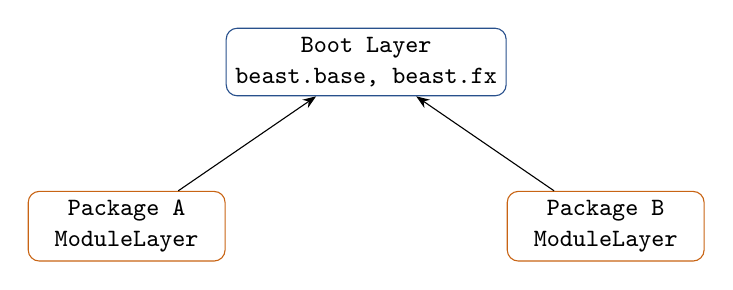
\begin{tikzpicture}[
    box/.style={draw=beastblue, rounded corners, minimum width=2.8cm, minimum height=0.8cm, font=\small\ttfamily, align=center},
    pkg/.style={draw=beastorange, rounded corners, minimum width=2.5cm, minimum height=0.8cm, font=\small\ttfamily, align=center},
    >=Stealth
]
\node[box] (boot) {Boot Layer\\beast.base, beast.fx};
\node[pkg, below left=1.2cm and 0cm of boot] (p1) {Package A\\ModuleLayer};
\node[pkg, below right=1.2cm and 0cm of boot] (p2) {Package B\\ModuleLayer};
\draw[->] (p1) -- (boot);
\draw[->] (p2) -- (boot);
\end{tikzpicture}
\end{center}

\begin{itemize}
\item Each deployed package gets its \textbf{own ModuleLayer}
\item No classpath conflicts between packages
\item Packages can have different versions of shared dependencies
\end{itemize}
\end{frame}

\begin{frame}{Maven Central Distribution}
\textbf{New:} packages can be published as plain Maven Central JARs.

\vspace{0.5em}
\begin{itemize}
\item Users install via BEAUti: \textbf{Install from Maven} button
\item Or CLI: \code{packagemanager -maven groupId:artifactId:version}
\item Resolution via Apache Maven Resolver
\item JARs cached in \code{\textasciitilde/.beast/2.8/maven-repo/}
\item Tracked in \code{maven-packages.xml}
\end{itemize}

\vspace{0.5em}
\begin{itemize}
\item Custom repos: \code{packagemanager -addMavenRepository <url>}
\item ZIP packages still work alongside Maven packages
\end{itemize}
\end{frame}

\begin{frame}{\code{beast-package-skeleton}}
Ready-to-copy template project on GitHub:

\vspace{0.5em}
\begin{itemize}
\item Maven \code{pom.xml} with BEAST 3 dependencies
\item \code{module-info.java} with \code{provides} declarations
\item Example \code{ScalarDistribution}, operator, and tests
\item BEAST XML using the strongly-typed spec API
\item Maven Central release profile (source, javadoc, GPG, publishing plugin)
\item \code{version.xml} JAR embedding
\end{itemize}

\vspace{1em}
\begin{exampleblock}{}
Start here: \url{https://github.com/CompEvol/beast-package-skeleton}
\end{exampleblock}
\end{frame}

% ============================================================
\section{Testing \& Dependencies}
% ============================================================

\begin{frame}{Testing Upgrades}
\begin{columns}[T]
\begin{column}{0.48\textwidth}
\textbf{JUnit 5}
\begin{itemize}
\item Primary framework (Jupiter 5.8.2)
\item JUnit 4 still compiles via vintage engine
\item \code{@Tag("slow")} for long MCMC tests
\item \code{mvn test} --- fast tests only
\item \code{mvn test -Pslow-tests} --- all
\end{itemize}
\end{column}
\begin{column}{0.48\textwidth}
\textbf{TestFX (GUI testing)}
\begin{itemize}
\item BEAUti tests run \textbf{headlessly}
\item Monocle Glass platform
\item No display server needed
\item TestFX 4.0.18 + JUnit 5 integration
\end{itemize}
\end{column}
\end{columns}
\end{frame}

\begin{frame}{Dependency Updates}
\begin{center}
\begin{tabular}{lll}
\toprule
\textbf{Dependency} & \textbf{BEAST 2} & \textbf{BEAST 3} \\
\midrule
Java & 8 / 11 & 25 \\
Build & Ant & Maven 3.9+ \\
Math & commons-math3 & commons-math4-legacy 4.0 \\
 & & + commons-numbers / rng / statistics \\
ANTLR & 4.x (bundled) & 4.13.2 (Maven) \\
JavaFX & bundled with JDK & 25.0.2 (Maven) \\
JUnit & 4 & 5 (Jupiter 5.8.2) \\
GUI tests & --- & TestFX 4.0.18 \\
\bottomrule
\end{tabular}
\end{center}
\end{frame}

\begin{frame}{BEAUti \& Templates}
\begin{itemize}
\item \textbf{fxtemplates namespacing} --- templates moved to module-unique paths (\code{beast.fx/fxtemplates/}) to avoid JPMS split-package conflicts
\item \textbf{Module resource scanning} --- \code{BeautiDoc} scans JPMS module resources, so templates are discovered from JARs on the module path
\item External packages use their own namespace:\\
  e.g.\ \code{beast.morph.models.fx/fxtemplates/}
\item Legacy path (\code{fxtemplates/*.xml}) still supported as fallback
\end{itemize}
\end{frame}

% ============================================================
\section{Summary}
% ============================================================

\begin{frame}{Migration Checklist}
\begin{enumerate}
\item \textbf{Update build} --- create \code{pom.xml} (or update Ant classpath JARs), target Java 25
\item \textbf{Fix compile errors} --- \code{StateNode} not \code{Function}, \code{scale()} removed, \code{Evaluator} gone
\item \textbf{Add \code{module-info.java}} --- declare \code{provides} for your \code{BEASTInterface} implementations
\item \textbf{Migrate to spec types} --- replace \code{RealParameter} inputs with \code{RealScalarParam} / \code{RealVectorParam} and domain types
\item \textbf{Update XML \& templates} --- use spec class names, new operator set, namespaced fxtemplates
\end{enumerate}
\end{frame}

\begin{frame}{Resources}
\begin{description}
\item[Migration guide] \code{scripts/migration-guide.md} --- class mapping tables, step-by-step instructions
\item[CHANGELOG] \code{CHANGELOG.md} --- full list of what changed and why
\item[Package skeleton] \url{https://github.com/CompEvol/beast-package-skeleton}
\item[BEAST 3 repo] \url{https://github.com/CompEvol/beast3}
\end{description}
\end{frame}

\end{document}
